\section{Bausteinsicht}
UML package and class diagrams (perhaps auto-generate with tool, but ensure clean and well-organized)
Include description of responsibility and name of each package and class.
List Externe Software used and provide links


\subsection{Games Importer Service}
\subsubsection{Klassendiagramm}
\graphic{GamesImporter}{Klassendiagramm des Game Importer Service}
\subsubsection{Verantwortlichkeiten}
Dieser Service ist dafür zuständig, die benötigten Daten bei der Riot API anzufragen und dann in der LoL Datenbank zu speichern. Die Struktur des Services ist im obigen Klassendiagramm zu sehen. \\
Die db Klasse bietet alle Funktionen, um mit der Datenbank zu interagieren: neue Daten speichern, Daten lesen und Daten updaten. Dazu wird das psycopg2 Package verwendet.\\
Die App Klasse beinhaltet den main loop (update\_loop Funktion). In dieser werden dann weitere Funktionen aufgerufen, um alle Spieler zu updaten. Dazu werden zuerst die Methoden des summoner.py Moduls verwendet, welche einen einzelnen Spieler updaten können. In dieser Methode werden zunächst alle Daten des Summoners (Level, Name, ...) aktualisiert. Dann wird das matchhistory.py Modul verwendet, welches für den Spieler die MatchHistory importieren kann (add\_missing\_games\_tp\_db(db, get\_match\_ids(), puuid). Dieses verwendet dabei noch die Challenges Klasse, welche die Challenges für einzelne Spieler speichern kann (store\_challenges()). Dabei werden mithilfe der in der Datenbank vorhandenen Werte für total, average und highscore die neuen Werte berechnet und diese dann gespeichert.\\

Der PlayerImportRequest erbt von der von GRPC generierten Klasse ImporterService und ist für die Verbindung mit der PlayerAPI zuständig. Über diese Klasse kann eine Anfrage gesendet werden, um den Import eines neuen Spielers zu starten, wobei dann dieselbe Abfolge durchlaufen wird wie oben bereits beim updaten eines Spielers beschrieben.

\subsubsection{Externe Software}
GRPC: \href{https://grpc.io/docs/languages/python/basics/}\\
Cassiopeia: \href{https://github.com/meraki-analytics/cassiopeia}\\
Riot Watcher: \href{https://github.com/pseudonym117/Riot-Watcher}\\
psycopg2: \href{https://pypi.org/project/psycopg2/}\\
Riot API: \href{https://developer.riotgames.com/}\\

\subsection{Player API}

\subsubsection{Komponentendiagramm}\label{subsubsec:player-api-component-diagram}

\begin{figure}
    \centering
    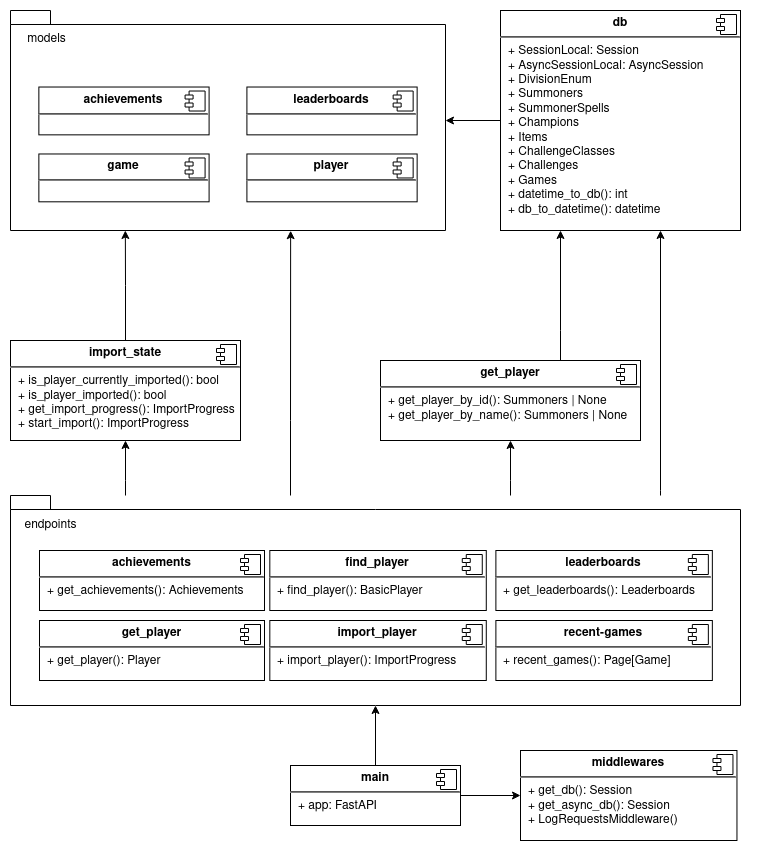
\includegraphics[width=\textwidth]{images/cdc-06-player-api-static.drawio}
    \caption{Komponenten Diagramm des PlayerAPI Services}
    \label{fig:player-api-component-diagram}
\end{figure}
Das in Abbildung~\ref{fig:player-api-component-diagram} abgebildete Komponenten Diagramm stellt die wichtigsten
Komponenten des PlayerAPI Services dar.
Wobei im \lstinline{model} Package nur die Module ohne die Klassen dargestellt werden, um das Diagramm
übersichtlich zu halten und es sich hierbei nur um Datenklassen handelt ohne Logik.

\subsubsection{Verantwortlichkeiten}

Dieser Service stellt folgende Endpunkte zur Verfügung:
\begin{itemize}
    \item \textbf{achievements}: Ein Spieler kann seine/ihre Challenges mit anderen Spielern vergleichen.
    \item \textbf{find\_player}: Prüft ob ein Spieler existiert.
    \item \textbf{leaderboards}: Stellt globale Highscore Listen zur Verfügung.
    \item \textbf{get\_player}: Stellt Informationen wie rank eines Spielers zur Verfügung
    \item \textbf{import\_player}: Triggert den Importprozess, falls Import noch nicht läuft.
    Gibt immer den aktuellen progress zurück.
    \item \textbf{recent\_games}: Stellt die zuletzt gespielten Spiele paginiert zur Verfügung.
\end{itemize}

Das \lstinline{main} Modul ist der Einstiegspunkt für die Applikation.
Hier wird die App mit den Routen konfiguriert, middlewares hinzugefügt und logging mit monitoring konfiguriert.

\lstinline{import_state} und \lstinline{get_player} haben Funktionen, die in fast jedem Endpunkt genutzt werden.

Im \lstinline{db} Modul ist das ORM Modell und die Verbindung zur Datenbank.

Das \lstinline{models} Package enthält Datenklassen, die keine Logik enthalten.
FastAPI wandelt diese in den Endpunkten automatisch in JSON um, wodurch alles typisiert ist.
Um das Diagramm übersichtlich zu halten, wurden nur die Module ohne die enthaltenen Klassen dargestellt.

\subsubsection{Externe Software}

\begin{itemize}
    \item \textbf{FastAPI} (\href{https://fastapi.tiangolo.com/}{https://fastapi.tiangolo.com/}): Web framework
    \item \textbf{pydantic} (\href{https://pydantic-docs.helpmanual.io/}{https://pydantic-docs.helpmanual.io/}): Datenklassen und Validierung
    \item \textbf{sqlalchemy} (\href{https://www.sqlalchemy.org/}{https://www.sqlalchemy.org/}): Datenbank ORM
    \item \textbf{GRPC} (\href{https://grpc.io/docs/languages/python/basics/}{https://grpc.io/docs/languages/python/basics/}): Kommunikation über GRPC
    \item \textbf{sentry} (\href{https://sentry.io}{https://sentry.io}): Fehler Überwachung fürs Monitoring
    \item \textbf{opentelemetry} (\href{https://opentelemetry.io/}{https://opentelemetry.io/}): Tracing fürs Monitoring
\end{itemize}

\subsection{User Management}
\subsubsection{Klassendiagramms}
\subsubsection{Verantwortlichkeiten}
Zu den eigenen Daten des User Backends gehören unter anderem die Region oder die Referenz zu einem Lol-Account dazu, 
aber auch alle notwendige Daten, die bei der Registrierung und beim Login entstehen. Für die Validierung dieser einkommenden Daten wurde die Libaries "Werkzeug" und "Marshmallow" verwendet.
Außerdem beinhaltet dieser Service die Zuständigkeit für das Token und Competitor Management. So wurde für das Kreieren und Validieren der Tokens die Libary
"PyJWT" verwendet.
\subsubsection{Externe Software}
\item \textbf{Flask} (\href{https://flask.palletsprojects.com/en/2.1.x/}{https://flask.palletsprojects.com/en/2.1.x/}): Webframework
\item \textbf{sqlalchemy} (\href{https://www.sqlalchemy.org/}{https://www.sqlalchemy.org/}): Datenbank ORM
\item \textbf{Werkzeug} (\href{https://pypi.org/project/Werkzeug/}{https://pypi.org/project/Werkzeug/}): Datenbank ORM
\item \textbf{Marshmallow} (\href{https://marshmallow.readthedocs.io/en/stable/}{https://marshmallow.readthedocs.io/en/stable/): Datenbank ORM
\item \textbf{PyJWT} (\href{https://pyjwt.readthedocs.io/en/latest/}{https://pyjwt.readthedocs.io/en/latest/}): Datenbank ORM

\newpage

\subsection{Frontend}

\subsubsection{Mockups}

Beim Planungsprozess wurden folgende Mockups erstellt.

\graphic{mockups/mockup_all.png}{lle Mockups des Frontends}

\subsubsection{Klassendiagramms}

\graphic{Frontend_UML.png}{Das UML-Diagramm des Frontends}

\subsubsection{Verantwortlichkeiten}

Die Benutzeroberfläche (Frontend) dient als Client und ist für die Kommunikation mit dem verschiedenen Microservices zuständig. Es stellt die Daten übersichtlich dar und sorgt für eine
angenehmes Nutzererlebnis. \\

\textbf{sign-up.vue}: Diese Seite ist für die Registrierung von neuen Benutzer:innen verantwortlich. Sobald die eine E-Mail und Passwörter übergeben wurden, so werden diese zunächst
validiert. Dies schließt die Überprüfung einer korrekten E-Mail-Adresse sowie die ausrechende Länge des Passwortes mit ein. Die Methode \verb|register()| sendet eine HTTP-Anfrage mit den 
entsprechenden Daten an das User-Backend, wo das Benutzerkonto erstellt wird.
\newline

\textbf{login.vue}: Zum Anmelden eines Benutzers muss auf dieser Seite die korrekten Anmeldedaten in das Formular eingegeben werden. Die Methode \verb|login()| prüft, ob das User-Backend
verifiziert hat, dass die Anmeldedaten korrekt sind. Ist dies der Fall, so wird der Token, das das User-Backend zusendet, gespeichert. 
\newline

\textbf{setting.vue}: Bei der ersten Anmeldung müssen die Nutzer:innen den gewünschten Spielernamen übergeben. Durch das Speichern dieser Einstellungen durch die Methode \verb|savePlayername|
sendet das Frontend den Spielernamen an das User-Backend. Anschließend werden die Nutzer:innen an die Hauptseite weitergeleitet. Im Zuge der Speicherung wird gleichzeitig ein "Import"-Befehl
an das "Player-Backend" gesendet, sodass die Spielerinformationen direkt importiert werden und zur Verfügung stehen. Die Methode \verb|deleteAccount| ist für das Löschen eines Kontos zuständig.
\newline

\textbf{index.vue}: Die Hauptseite stellt mithilfe der Methode \verb|fetchRandomStats| Leaderboard-Statistiken dar. Hierfür das "Player-Backend" angefragt, welches zufällige 
Leaderboards zurückgibt.
\newline

\textbf{dashboard.vue}: Das Dashboard stellt alle Informationen zu der jeweiligen LOL-Spieler:in dar. Die Methode \verb|fetchUserData| ruft die Spielerdaten anhand des gespeicherten Tokens
von dem "Player-Backend" ab. Ebenso wird geprüft, ob die Account bereits importiert wird. Ist das nicht der Fall, so wird ein Ladebalken dargestellt, der den Import-Fortschritt aufzeigt. Dies
wird durch eine regelmäßige Anfrage an das "Player-Backend" ermöglicht, welches die Aktuellen importieren Spiele sowie den Fortschritt in Prozent zurückgibt.
\newline

\textbf{competitors.vue}: Auf der "Competitors"-Seite können Spieler:innen zum Vergleichen von Statistiken hinzugefügt oder gelöscht werden. Die Methode \verb|getCompetitors| ruft die gespeicherten
Freunde des Spielers ab und listet sie auf. Die Methode \verb|removeCompetitor| entfernt den jeweiligen Gegner aus der Freundesliste.
\newline

\textbf{achievements.vue}: Auf dieser Seite kann der eigene Account mit anderen Personen oder Ranks verglichen werden. Die einzelnen "Challanges" werden in Tabellen aufgelistet und in Tabs unterteilt.
Das Aufrufen der Seite führt die Methode \verb|fetchAchievements| aus, die eine Anfrage an das "Player-Backend" sendet. Mithilfe eines Filtersystems können die persönlichen
Statistiken zwischen den Freundeslisten, Global oder nur mit einer gewünschten Person verglichen werden. Falls der zu vergleichende Spieler nicht importiert wurde, kann auch von dort dieser über einen 
Button importiert werden, wodurch die Methode \verb|importPlayer| aufgerufen wird. Außerdem ist es möglich, bestimmte Kategorien als Favorit abzuspeichern. Diese übernimmt die Methode
\verb|toggleFavoriteAchivement|, die beim Betätigen der Favoriten-Buttons ausgelöst wird. Die Methode \verb|filterApplied| sendet eine aufbereitete HTTP-Anfrage mit den entsprechenden Filtern
an das "Player-Backend", sobald die gewünschten Filter übernommen wurden.
\newline

\subsubsection{Externe Software}